\normalfalse \difficilefalse \tdifficiletrue
\correctionfalse

%\UPSTIidClasse{11} % 11 sup, 12 spé
%\newcommand{\UPSTIidClasse}{12}

\exer{Maxpid $\star\star\star$ \label{C2:06:18}}
\setcounter{question}{0}\UPSTIcompetence[2]{C2-06}
\index{Compétence C2-06}
\index{Maxpid}
\ifcorrection
\else
\marginnote{\textbf{Pas de corrigé pour cet exercice.}}
\fi

\ifprof
\else

Soit le schéma suivant. 
\begin{center}
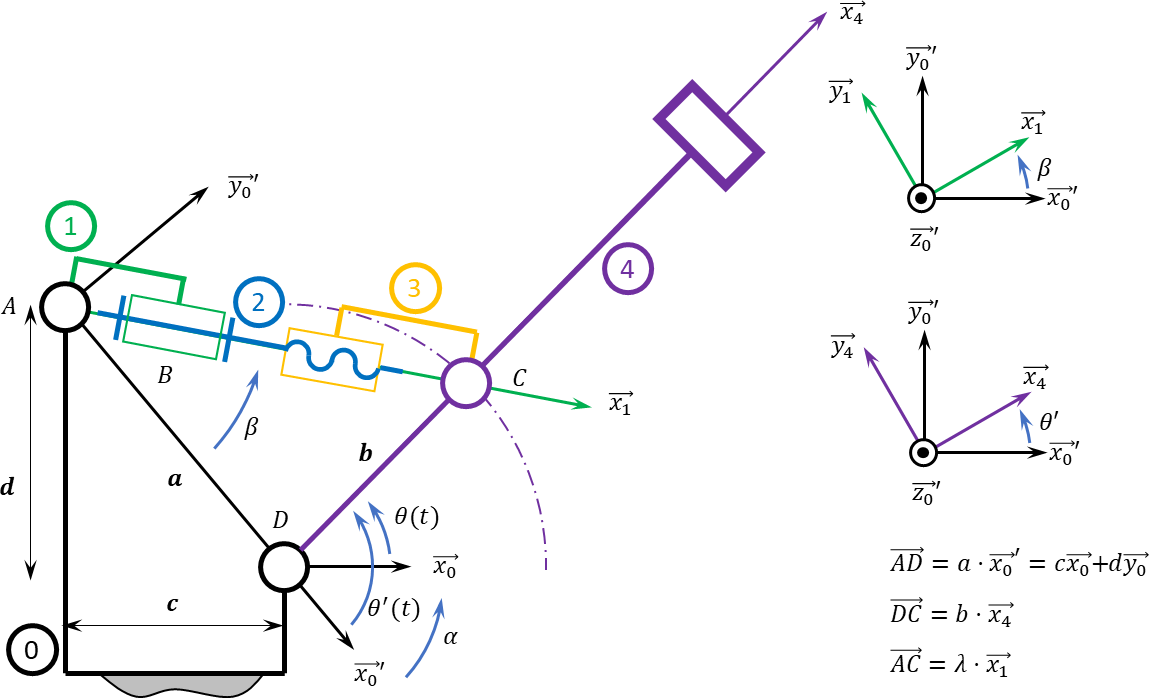
\includegraphics[width=\linewidth]{18_01}
\end{center}
\fi

Par ailleurs $a=\SI{107,1}{mm}$, $b=\SI{80}{mm}$, $c=\SI{70}{mm}$, $d=\SI{80}{mm}$. Le pas de la vis est de $\SI{4}{mm}$.

\question{Tracer le graphe des liaisons.}
\ifprof
\else

\fi\question{Exprimer $ \theta(t)$ en fonction de $\lambda(t)$.}
\ifprof
\else
\fi

\question{Exprimer $\dot{\theta}(t)$ en fonction de $\dot{\lambda}(t)$.}
\ifprof
\else
\fi

\question{Exprimer $\dot{\theta}(t)$ en fonction de ${\omega}(t)$, vitesse de rotation du rotor moteur \textbf{2} par rapport au stator \textbf{1}.}
\ifprof
\else
\fi

\question{En utilisant Python, tracer $\dot{\theta}(t)$ en fonction de ${\omega}(t)$. On considérera que la fréquence de rotation de la pièce \textbf{2} par rapport à \textbf{1} est de 500 tours par minute.}
\ifprof
\else
\fi


\ifprof
\else
\begin{flushright}
\footnotesize{Corrigé  voir \ref{C2:06:18}.}
\end{flushright}%
\fi